\section{Linear Discriminant Analysis}
Using Linear Discriminant Analysis\footnote{\cite{James2013} p. 138} (LDA) one can overcome several problems with logistic regression. When the classes are well-separated, the parameter estimates for the logistic regression model are unstable. If our sample size is small and the distribution of the predictors X is a normal distribution in each of the classes, the linear discriminant model is more applicable than the logistic regression model.
\subsection{Theory}
Before one start using LDA there is a  assumption about the data it operates on. Each of the predictors should be normally distributed. The formula used by LDA is shown in Equation \ref{fo:BayesTheorem}. Where $\pi_k$ is the prior probability that a randomly selected observation comes from the $k$'th class. $f_k(x)$ is the probability density function of X for an observation that comes from the $k$'th class. If the result is large then there is a high probability that an observation is predicted to be in the $k$'th class.
\begin{align}\label{fo:BayesTheorem}
Pr(Y=k|X=x) = \frac{\pi_k f_k(x)}{ \sum_{l=1}^{k}\pi_l f_l(x) }
\end{align}
If we as an example choose to only use one predictor and we would like to obtain the estimate for $f_k(x)$ that we can use in Equation \ref{fo:BayesTheorem}. Assuming that $f_k(x)$ is normally distributed and assuming that the variance is the same for all $k$'th classes, the result is Equation \ref{fo:BayesTheoremWithNormal}.
\begin{align}\label{fo:BayesTheoremWithNormal}
P_k(x) = \frac{\pi_k \frac{1}{\sqrt{(2\pi\sigma)}}\exp(-\frac{1}{2\sigma^2}(x-\mu_k)^2)}{\sum_{l=1}^{k}\pi_l \frac{1}{\sqrt{(2\pi\sigma)}}\exp(-\frac{1}{2\sigma^2}(x-\mu_l)^2) }
\end{align}
If we then take the log of Equation \ref{fo:BayesTheoremWithNormal} and manipulate the terms we will arrive at Equation \ref{fo:BayesTheoremAfterManipulateTheterms} this is the same as assigning the observation to the class for which it is largest.
\begin{align}\label{fo:BayesTheoremAfterManipulateTheterms}
\delta_k = x\frac{\mu_k}{\sigma^2} - \frac{\mu^2_k}{2 \sigma^2} + \log(\pi_k)
\end{align}
In the example seen in Figure \ref{fig:TwoOneDimensionalNormalDensityFunctions}\footnote{\cite{James2013} p. 140} The two probability density functions (PDF), $f_1(x)$ and $f_2(x)$, represent two distinct classes. The mean and variance parameters for the two density functions are $\mu=-1.25 \mu_2=1.25$ and $\sigma^2_1=\sigma^2_2=1$
\begin{figure}[H]
	\centering
	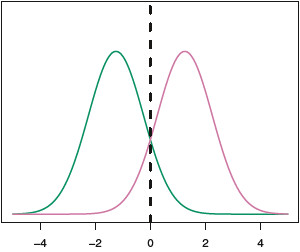
\includegraphics[scale=2.0]{discriminantAnalysis/linearDiscriminantAnalysis/fig/TwoOneDimensionalNormalDensityFunctions.jpg}
	\caption{Two normal distributions with the Bayes decision boundary in the middle.}
	\label{fig:TwoOneDimensionalNormalDensityFunctions}
\end{figure}


\subsection{Results}
\subsubsection*{LAB 4.6.3}
<<<<<<< Updated upstream
The lab 4.6.3\footnote{Appendix 5 - 4.6.3 Linear Discriminant Analysis} is using LDA. As shown in lab 4.6.2 the data is split into before and after 2005, a training and testing set. Afterwards the LDA is imported from scikit-learn.
=======
The lab 4.6.3 is using LDA. As shown in lab 4.6.2 the data is split into before and after 2005, a training and testing set. Afterwards the LDA is imported from scikit-learn.
>>>>>>> Stashed changes

Now that the model have been fitted it will look at the coefficients of the model for Lag1 and Lag2.

\noindent\textit{Lag1: $-0.05544078$\\
Lag2: $-0.0443452$}

With the following data $\hat{ \pi }_1 = -0.05544078$ and $\hat{ \pi }_2 = -0.0443452 $, results in the priors:%TODO problematic

\noindent\textit{0.49198397\\
0.50801603}

Testing the model on the test data results in an accuracy of $0.55952380952380953$ approximately $0.56$.

Changing the threshold to test for improvements in the accuracy. The 2nd column of X\_test\_prob is the probability belongs to UP group. The default value is $0.50$, changing this to $0.48$ result in $0.56349206349206349$ approximately $0.56$.
